
%%%%%%%%%%%%%%%%%%%%%%% file typeinst.tex %%%%%%%%%%%%%%%%%%%%%%%%%
%
% This is the LaTeX source for the instructions to authors using
% the LaTeX document class 'llncs.cls' for contributions to
% the Lecture Notes in Computer Sciences series.
% http://www.springer.com/lncs       Springer Heidelberg 2006/05/04
%
% It may be used as a template for your own input - copy it
% to a new file with a new name and use it as the basis
% for your article.
%
% NB: the document class 'llncs' has its own and detailed documentation, see
% ftp://ftp.springer.de/data/pubftp/pub/tex/latex/llncs/latex2e/llncsdoc.pdf
%
%%%%%%%%%%%%%%%%%%%%%%%%%%%%%%%%%%%%%%%%%%%%%%%%%%%%%%%%%%%%%%%%%%%


\documentclass[runningheads,a4paper]{llncs}

\usepackage{amssymb}
\setcounter{tocdepth}{3}
\usepackage{graphicx}
%\usepackage{natbib}
\usepackage{tikz}
%\usepackage{hyperref}
\usetikzlibrary{arrows}
\usepackage{fancyeq}

\newcommand{\citep}[1]{\cite{#1}}
\newcommand{\citet}[1]{\cite{#1}}

\usepackage{xcolor}
\newcommand{\todo}[1]{[{\color{blue}#1}]}

\usepackage{url}
\urldef{\mailsa}\path|{alfred.hofmann, ursula.barth, ingrid.haas, frank.holzwarth,|
\urldef{\mailsb}\path|anna.kramer, leonie.kunz, christine.reiss, nicole.sator,|
\urldef{\mailsc}\path|erika.siebert-cole, peter.strasser, lncs}@springer.com|    
\newcommand{\keywords}[1]{\par\addvspace\baselineskip
\noindent\keywordname\enspace\ignorespaces#1}

\newcommand {\lbrac} {\makebox[0pt]{[\kern-1ex[}}
\newcommand {\rbrac} {\makebox[0pt]{]\kern-1ex]}}
\newcommand{\denote}[1]{\lbrac~#1~\rbrac}

\tikzstyle{int}=[draw, minimum size=2em]
\tikzstyle{init} = [pin edge={thin,gray}]

\begin{document}

\mainmatter  % start of an individual contribution

% first the title is needed
\title{A tale of two abstractions:\\Monad transformers and object-orientation}

% Monads: the world's finest object-oriented programming language
% Exploring object-oriented programming with monads
% Functional programming: the world's finest object-oriented programming language

% a short form should be given in case it is too long for the running head
%\titlerunning{Programming with monadic state hierarchies}

% the name(s) of the author(s) follow(s) next
%
% NB: Chinese authors should write their first names(s) in front of
% their surnames. This ensures that the names appear correctly in
% the running heads and the author index.
%
\author{Michael B. Gale \and Alan Mycroft}
%
%\authorrunning{Lecture Notes in Computer Science: Authors' Instructions}
% (feature abused for this document to repeat the title also on left hand pages)

% the affiliations are given next; don't give your e-mail address
% unless you accept that it will be published
\institute{Computer Laboratory, University of Cambridge}

%
% NB: a more complex sample for affiliations and the mapping to the
% corresponding authors can be found in the file "llncs.dem"
% (search for the string "\mainmatter" where a contribution starts).
% "llncs.dem" accompanies the document class "llncs.cls".
%

\toctitle{Lecture Notes in Computer Science}
\tocauthor{Authors' Instructions}
\maketitle


\begin{abstract}
%We present an encoding of the principal features of object-oriented languages in pure Haskell. Our system supports object classes, inheritance, subtype polymorphism, dynamic dispatch, and open recursion. We establish a correspondence between inheritance and monad transformers by defining a state monad transformer for each class, parametrised only over the class's own state. The methods of a class are monadic computations which run on top of a stack of monad transformers, consisting of one layer for the class and each of its ancestors. Well-known limitations of monad transformers are overcome by the dynamic dispatch mechanism. The encoding allows class hierarchies to be open for extension in separately-compiled modules, therefore allowing the construction of modular programs. We show how to translate to our encoding from a small object-oriented language. Finally, we provide a Template Haskell implementation of this translation.

%Monad transformers are infamous for being awkward to work with. By only considering state monad transformers, we show that there exists a correspondence to the usual inheritance mechanism of object-oriented languages. While such languages take care of the boilerplate required for inheritance to work seamlessly, this is not the case for monad transformers. We exploit this correspondence and combine state monad transformers with the principal features of object-oriented languages, allowing us to treat stacks of state monad transformers like objects. We illustrate using examples that these objects are as easy to work with as their counterparts in object-oriented languages. Additionally, if we extend our system with an encoding for subtyping, we are able to write modular programs. Our system is encoded entirely in Haskell and requires no new language features. A Template Haskell library allows programmers to write class definitions in the same style as in object-oriented languages which then get translated to the corresponding encodings. We hope that our findings will form the foundation for a generalised system in which classes can have effects other than state.


Monad transformers are infamous for being awkward to work with. To begin tackling this problem, we formulate a correspondence between state monad transformers and the inheritance mechanism of object-oriented languages. While object-oriented languages implicitly supply the boilerplate required for inheritance to work seamlessly, state monad transformers require it to be explicit. By hiding this boilerplate in type class instances, we simulate the dispatch mechanisms of object-oriented languages. This allows us to use stacks of state monad transformers as easily as objects. We illustrate using examples that these `objects' are as easy to work with as their object-oriented counterparts.

Our `object classes' do not need to know about other `object classes' which inherit from them. The resulting hierarchy is therefore open for extension. This can be taken advantage of to construct modular data types and programs through the addition of an encoding for subtyping. All of this is encoded entirely in Haskell and requires no new language features. Finally, a Template Haskell library allows programmers to write class definitions in the same style as in object-oriented languages from which the boilerplate can automatically be derived.



%This opens up an exciting new 
%By establishing the effect of monad transformers to be a generalised form of inheritance, we show that state monad transformers can be used as natural interpreters for an object-oriented language. 

 

\keywords{Haskell, Monad Transformers, Object-Oriented Programming}
\end{abstract}

\section{Introduction}
\label{sec:introduction}

In a purely-functional programming language, such as Haskell, we might wish to write an application which interacts with an in-memory database. Since values are immutable, an update to the database returns a new, updated copy of it. To avoid having to keep track of the most recent version of the database, we use the state monad:
\begin{displaymath}
\begin{array}{lcl}
\multicolumn{3}{l}{\mathbf{type}~\mathit{Database} = \mathit{StateT}~\mathit{SqlDatabase}~\mathit{Identity}}\\
\mathit{runQuery} & :: & \mathit{String} \to \mathit{Database}~\mathit{SqlReader}
\end{array}
\end{displaymath}
If given an SQL query, represented as a string of characters, $\mathit{runQuery}$ will run it using the underlying database. The database is represented by the $\mathit{SqlDatabase}$ type and is wrapped into a state monad transformer, giving us the effect of mutability. 

Writing an application just using $\mathit{runQuery}$ may be prone to errors, however. For example, if the name of a table or column changes, all queries which refer to it must be updated as well. A common solution for this is to abstract over the entity model of the database instead of writing SQL queries directly. For this purpose, we define a data type which represents our entity model. In this example, we have a table containing recipes, indexed by a unique, numeric identifier:
\begin{displaymath}
\begin{array}{lcl}
\multicolumn{3}{l}{\mathbf{data}~\mathit{Model} = \mathit{MkModel}~(\mathit{Map}~\mathit{Int}~\mathit{Recipe})}
\end{array}
\end{displaymath}
The model caches all changes we make to the table and only updates the database when we wish to do so. To implement this, we layer the model on top of the database using the state monad transformer:
\begin{displaymath}
\begin{array}{lcl}
\multicolumn{3}{l}{\mathbf{type}~\mathit{DbModel} = \mathit{StateT}~\mathit{Model}~\mathit{Database}}\\\\
\mathit{saveChanges} & :: & \mathit{DbModel}~() \\
\mathit{saveChanges} & = & \mathbf{do} \\
\multicolumn{3}{l}{\qquad \begin{array}{lcl}
    m & \leftarrow & \mathit{get} \\
    \multicolumn{3}{l}{\mathbf{let}} \\
    \multicolumn{3}{l}{\qquad \mathit{query} = \ldots} \\
    \multicolumn{3}{l}{\mathit{lift}~(\mathit{runQuery}~\mathit{query})}
\end{array} }
\end{array}
\end{displaymath}
The $\mathit{saveChanges}$ function is responsible for updating the database according to the cached changes. To use this implementation, we might write the following:
\begin{displaymath}
\begin{array}{l}
\mathit{runState}~(\mathit{runStateT}~\mathit{go}~\mathit{emptyModel})~\mathit{initialDatabase} \\
\qquad \mathbf{where} \\
\qquad \qquad \begin{array}{lcl}
\mathit{go} & = & \mathbf{do}~\{ \mathtt{\{-~do~work~-\}}~\mathit{saveChanges} \}
\end{array}
\end{array}
\end{displaymath}
One way of interpreting the $\mathit{runState}$ and $\mathit{runStateT}$ functions is as the equivalent of opening a new scope in a language like C, which causes additional variables to be stored on the stack. The calls to $\mathit{lift}$ correspond to following indirections on the stack to locate variables. Another way of viewing this behaviour is as inheritance as we know it from object-oriented programming: the outer state monad transformer has access to the inner state monad transformer's state. $\mathit{lift}$ is then like an explicit $\mathit{super}$ in Java or $\mathit{base}$ in C\#.

Neither interpretation requires the programmer to explicitly implement this behaviour in other languages, yet it has to be made explicit for monad transformers in Haskell. We believe that this is at least partially due to the lack of names in monad stacks, while local variables in C and class members in object-oriented languages both have names. In Haskell's \texttt{mtl} library, type classes are used to allow for the automatic lifting of functions such as $\mathit{get}$ and $\mathit{put}$ through a monad stack, if there is only one state monad in it. In other words, it addresses the naming problem for distinct effects, but not for several instances of the same effect.

Interestingly, if we add names to the computations which can be run on a monad stack, then we run into the expression problem. [I need to explain this more]

In this work, we treat stacks of state monad transformers as objects and allow programmers to define classes of state monad transformer stacks. Specifically, our contributions are:
\begin{itemize}
    \item We have established a relationship between inheritance and (state) monad transformers. This relationship also leads to similarities to the expression problem.
    \item State monad transformers have had this behaviour all along, but thus far it has been awkward for programmers to make use of it. We show how to encode a simple object system in Haskell which exploits the correspondence to inheritance to simplify the usage of state monads -- chapter 2
    \item By adding subtyping to our system, we enable a third type of polymorphism within Haskell. In addition to the existing parametric polymorphism and ad-hoc polymorphism, subtype polymorphism enables programmers to construct modular data types. Our approach does not require whole-program compilation unlike, for example, open data types and functions \cite{loh2006open} -- chapter 3
    \item We use Template Haskell to provide a convenient method for programmers to generate such encodings from class definitions without any new extensions to the host language. We require no transformation of any function or method definitions as our library implements the combinators in standard Haskell -- chapter 4
\end{itemize}

\textbf{-- OLD INTRODUCTION --}

Different programming paradigms evolve independently, but occasionally cross-pollination takes place. Features characteristic of the functional paradigm, such as \emph{e.g.} anonymous and higher-order functions, have made their way into object-oriented languages such as \emph{e.g.} C\# and Java 8. Often this cross-pollination highlights other issues. For example, immutability is useful for functional constructs but hard to express in Java. Similarly, work combining functional and logic programming \citep{nadathur1988overview,hanus2006curry,somogyi1996execution} helped us better understand interactions of backtracking and laziness, and higher-order functions and unification.

In this work, we encode object-oriented features in a purely functional language, namely Haskell. Doing so not only allows programmers to explore new ways of structuring functional programs, but also casts light in the opposite direction---adding a new point in the old object-oriented debate concerning the difference between subtyping and inheritance \cite{cook1989inheritance}. 

For convenience, we present syntactic sugar for our object system on top of standard Haskell. This de-sugars back to pure Haskell and monads in a way entirely
parallel to the way that Haskell's $\mathbf{do}$-notation does for imperative code.

Object-oriented programming as a paradigm describes a range of related concepts in the same way that functional programming does. However, languages which associate themselves with one paradigm rarely support all of its characteristic features. \citet{armstrong2006quarks}, for example, surveys object-oriented languages in an attempt to identify what concepts characterise object-oriented programming. According to Armstrong, some of the most common features in such languages are: dynamic dispatch, encapsulation, subtype polymorphism, and inheritance. 

It is already folklore that dynamic dispatch can be implemented in Haskell with existential types and type classes. In the following example, a value of type $\mathit{Bird}$ is constructed by applying the $\mathit{MkBird}$ constructor to some type $a$ for which there is an instance of the $\mathit{BirdLike}$ type class:
\begin{displaymath}
\begin{array}{lcl}
\mathbf{data}~\mathit{Bird} & = & \forall a. \mathit{BirdLike}~a \Rightarrow \mathit{MkBird}~a
\end{array}
\end{displaymath}
The $\mathit{Bird}$ type effectively serves as an abstract base class. It is not possible to obtain a value of this type without some other type $a$ which implements $\mathit{BirdLike}$. Any such type can be seen as a subtype of $\mathit{Bird}$ and type-casts to the base class are possible by applying the $\mathit{MkBird}$ constructor. The type class constraint ensures that every subtype has the properties we would expect of, in this example, a bird.

This is an intriguing concept, but is often perceived as an anti-pattern. After all, why should we bother with a base class type if we can simply place a type class constraint on every function expecting bird-like arguments and avoid the $\mathit{Bird}$ type all-together?

We answer this question and show how the above concept can be elevated from a neat trick without much practical use to the foundation of an object system for purely-functional languages with a range of benefits. Specifically, our contributions are:
\begin{itemize}
    \item We build upon the technique of using existential types combined with type classes to encode a comprehensive object system in Haskell, supporting object classes, inheritance, coercive subtype polymorphism, and non-aliased mutation. In Section \ref{sec:usage} we first show how objects in our encoding are used within a standard Haskell program, before describing the encoding itself in Section \ref{sec:encoding}.
    \item Class hierarchies in our encoding are open for extension and do not require whole-program compilation. We thereby improve upon approaches which do, such as \emph{e.g.} open data types and functions \cite{loh2006open}.
    \item Our system enables open recursion, allowing methods of one object class to call other methods which have either no implementation (\emph{i.e.} are abstract) or are overriden by a deriving class.
    %\item Monad transformers \cite{moggi1989abstract,jones1995transformers} allow monadic effects to be layered on top of each other to form ``monad stacks''. Functions which make use of the effects in this stack cannot always be called directly, however. If a function's effect does not match that of the whole stack, programmers must indicate explicitly how many layers would have to be taken off in order for it to match. In Haskell, this is accomplished by wrapping a function in a call to $\mathit{lift}$ for every monad in a stack of monad transformers that should be skipped. Our system hides this boilerplate in the dynamic dispatch mechanism. 
    \item We show how to translate from a simple notation for object classes, following the conventions of object-oriented languages, to the corresponding encodings in Haskell (Section \ref{sec:auto}).
    \item This translation is implemented as a Haskell library using Template Haskell combined with a suitable set of combinators (Section \ref{sec:th}).
\end{itemize}
\section{Monad stacks and object-orientation}

Consider the database example from Section 1. As the programmer, we know when writing the $\mathit{saveChanges}$ function that $\mathit{runQuery}$ can be run on a smaller part of our monad stack. \emph{I.e.} it requires the monad stack to be $\mathit{State}~\mathit{SqlDatabase}$, while the monad stack of $\mathit{saveChanges}$ also provides more state on top of that. As a result of this type incompatibility, we must use $\mathit{lift}$ to execute, in this case, the $\mathit{runQuery}$ function on the layer of the monad stack which corresponds to the one expected by $\mathit{runQuery}$. If this layer is multiple levels away from the top of the stack, multiple, successive calls to $\mathit{lift}$ are required.

Let us refer to function calls where a monad stack has already been set up as \emph{internal calls} as opposed to \emph{external calls} where a monad stack has not yet been set up using the required $\mathit{runX}$ functions, such as \emph{e.g.} $\mathit{runStateT}$. We will address external calls later in this section. 

\subsection{Internal calls}

Most monadic computations in Haskell are represented by values of some data type which are combined with $\bind$ and ultimately evaluated by some corresponding $\mathit{runX}$ function. Monad stacks are therefore just nested data types. A monadic computation, such as $\mathit{runQuery}$ returns a value of the data type corresponding to the monad stack it runs on. Since $\mathit{runQuery}$ and $\mathit{saveChanges}$ run on top of different monad stacks, they return values of different, incompatible types. In order to use $\mathit{runQuery}$ on top of the same monad stack as $\mathit{saveChanges}$, it must return a value of the same type. In other words, we really want $\mathit{runQuery}$ to be an overloaded function which returns a value of the data type corresponding to the context in which it is called. Overloading in Haskell is achieved through type classes, so instead of defining $\mathit{runQuery}$ as a global function with a specific type, we should instead define it as part of a type class:
\begin{displaymath}
\begin{array}{l}
\mathbf{class}~\mathit{SqlDatabaseCtx}~m~\mathbf{where}\\
\qquad \begin{array}{lcl}
\mathit{runQuery} & :: & \mathit{String} \to m~\mathit{SqlReader}
\end{array}
\end{array}
\end{displaymath}
This type class has a single parameter $m$ which represents the context in which $\mathit{runQuery}$ should be callable. In other words, $m$ should be the data type which corresponds to a monad stack on top of which $\mathit{runQuery}$ can be run. To restore the old functionality, we must provide an instance for $\mathit{SqlDatabaseCtx}$ for the most basic monad stack on top of which $\mathit{runQuery}$ can be run\footnote{Note that this requires the \texttt{FlexibleInstances} language extension.}:
\begin{displaymath}
\begin{array}{l}
\mathbf{instance}~\mathit{SqlDatabaseCtx}~\mathit{MyDatabase}~\mathbf{where}\\
\qquad \begin{array}{lcl}
\mathit{runQuery}~\mathit{query} & = & \ldots
\end{array}
\end{array}
\end{displaymath}
We once again omit the exact definition of $\mathit{runQuery}$, but it remains unchanged from the previous implementation. In order to call $\mathit{runQuery}$ from the extended monad stack used by $\mathit{saveChanges}$, we need a second instance for its monad stack:
\begin{displaymath}
\begin{array}{l}
\mathbf{instance}~\mathit{SqlDatabaseCtx}~\mathit{DbModel}~\mathbf{where}\\
\qquad \begin{array}{lcl}
\mathit{runQuery}~\mathit{query} & = & \mathit{lift}~(\mathit{runQuery}~\mathit{query})
\end{array}
\end{array}
\end{displaymath}
We can now rewrite the definition of $\mathit{saveChanges}$ to get rid of the explicit call to $\mathit{lift}$:
\begin{displaymath}
\begin{array}{lcl}
\mathit{saveChanges} & :: & \mathit{DbModel}~() \\
\mathit{saveChanges} & = & \mathbf{do} \\
\multicolumn{3}{l}{\qquad \begin{array}{lcl}
    m & \leftarrow & \mathit{get} \\
    \multicolumn{3}{l}{\mathbf{let}} \\
    \multicolumn{3}{l}{\qquad \mathit{query} = \ldots} \\
    \multicolumn{3}{l}{\mathit{runQuery}~\mathit{query}}\\
    \multicolumn{3}{l}{\mathit{return}~()}
\end{array} }
\end{array}
\end{displaymath}

\textbf{TODO: Some concluding remarks about names; relation to the expression problem}\\
\textbf{TODO: Say something about monad stacks being ``interpreters'' for inheritance}

\subsection{Monad stack configurations}

Since monadic computations are just values of some data type, they cannot just be evaluated like a regular function. Instead, each monad $X$ has a corresponding $\mathit{runX}$ function which can be used to evaluate a computation. If we have a stack of monads, then successive calls to these functions are required for each layer in the stack, as shown in Section 1. This is often cumbersome as the programmer has to remember to insert the calls to these $\mathit{runX}$ functions, place them in the right order, and supply them with the right arguments.

Let us introduce a notation of \emph{monad stack configurations} or, more simply, ``objects''. An object in our system is a value which, when supplied to an external call, provides all the required information to set up an appropriate monad stack for that computation. In other words, the external call first becomes an interpreter for the object which calls the appropriate $\mathit{runX}$ functions in an order specified by the object, before making the internal call corresponding to itself on top of the newly constructed monad stack. Finally, the external call will return an updated object as well as a result. For this paper, we will only consider objects corresponding to state monads,

Before we look at the behaviour of external calls in detail, let us define the structure of objects. Objects are represented using an algebraic data type. \textbf{TODO: explain what a class is} For a base class -- a class which has no ancestors -- there is only one possible data constructor. For the $\mathit{MyDatabase}$ monad from our running example, we would have:
\begin{displaymath}
\begin{array}{lcl}
\mathbf{data}~\mathit{MyDatabaseObj} & = & \mathit{MkMyDatabaseData}~\{ \\
\multicolumn{3}{l}{\qquad \mathit{myDatabaseState} :: \mathit{SqlDatabase} }  \\
\} && 
\end{array}
\end{displaymath}

\begin{displaymath}
\begin{array}{lcl}
\mathbf{data}~\mathit{DbModelObj} & = & \mathit{MkDbModelData}~\{ \\
\multicolumn{3}{l}{\qquad \begin{array}{lcl}
\mathit{dbModelParent} & :: & \mathit{MyDatabaseObj}, \\
\mathit{dbModelState} & :: & \mathit{Map}~\mathit{Int}~\mathit{Recipe}
\end{array}  }  \\
\} && 
\end{array}
\end{displaymath}

\subsection{External calls}

\begin{displaymath}
\begin{array}{l}
\mathbf{class}~\mathit{SqlDatabaseCtx}~\mathit{obj}~\mathit{st}~m \mid \mathit{obj} \to \mathit{st}, \mathit{st} \to \mathit{obj}~\mathbf{where}\\
\qquad \begin{array}{lcl}
\mathit{runQuery\_int} & :: & \mathit{String} \to \mathit{StateT}~\mathit{st}~m~\mathit{SqlReader} \\
\mathit{runQuery\_ext} & :: & \mathit{obj} \to \mathit{String} \to m~(\mathit{SqlReader}, \mathit{obj})
\end{array}
\end{array}
\end{displaymath}
\section{Subtyping}
\label{sec:encoding}

A pleasant property of class hierarchies in object-oriented languages is that they are open for extension. In other words, classes do not need to know about other classes which inherit from them. For example, consider the following, abstract base class for an expression language in Java:
\begin{displaymath}
\begin{array}{l}
\mathbf{abstract}~\mathbf{class}~\mathit{Expr}~\{\\
\qquad \mathbf{public}~\mathbf{abstract}~\mathit{int}~\mathit{eval}();\\
\}
\end{array}
\end{displaymath}
This roughly corresponds to an algebraic data type $\mathit{Expr}$ in Haskell with no constructors and a function $\mathit{eval} :: \mathit{Expr} \to \mathit{Int}$. However, while we cannot retrospectively add constructors to a data type in Haskell, we can extend the $\mathit{Expr}$ class in Java:
\begin{displaymath}
\begin{array}{l}
\mathbf{class}~\mathit{Val}~\mathbf{extends}~\mathit{Expr}~\{\\
\qquad \mathbf{private}~\mathit{int}~\mathit{value};\\\\
\qquad \mathbf{public}~\mathit{int}~\mathit{eval}()~\{\\
\qquad \qquad \mathbf{return}~\mathit{this}.\mathit{value};\\
\qquad \}\\
\}
\end{array}
\end{displaymath}
The author of the $\mathit{Expr}$ class does not need to know about the $\mathit{Val}$ class and may even compile a library only containing $\mathit{Expr}$. The class can still be extended in other libraries by other authors, however. Our object system from Section \ref{sec:objects} allows for the same, but it has one major limitation: there is no support for subtyping that would allow us to \emph{e.g.} cast a $\mathit{DbModel}$ object to a $\mathit{MyDatabase}$ object. To see why this is an important limitation, consider the following sub-class for $\mathit{Expr}$ in Java:
\begin{displaymath}
\begin{array}{l}
\mathbf{class}~\mathit{Add}~\mathbf{extends}~\mathit{Expr}~\{\\
\qquad \mathbf{private}~\mathit{Expr}~\mathit{left};\\
\qquad \mathbf{private}~\mathit{Expr}~\mathit{right};\\\\
\qquad \mathbf{public}~\mathit{int}~\mathit{eval}()~\{\\
\qquad \qquad \mathbf{return}~\mathit{this}.\mathit{left}.\mathit{eval}() + \mathit{this}.\mathit{right}.\mathit{eval}();\\
\qquad \}\\
\}
\end{array}
\end{displaymath}
Without subtyping, the $\mathit{Add}$ class would be useless. There would be no possible values for the $\mathit{left}$ and $\mathit{right}$ fields, since $\mathit{Expr}$ itself is abstract and cannot be instantiated. It is only useful if sub-classes of $\mathit{Expr}$, which can be instantiated, can be used as $\mathit{Expr}$ values. In the remainder of this section, we show how to modify the encodings for our object system to support \emph{coercive subtyping} in Haskell.

\subsection{Objects as heterogenous zippers}

Objects so far have been represented using what are essentially singly-linked lists of $\Delta$-objects in which the $\Delta$-objects of sub-classes store their parent's $\Delta$-object. This in turn may contain its parent's $\Delta$-object, and so on. This is easy, because sub-classes always know the type of their parent. The inverse, however, is not true. Parental classes do not know what their children are. In order to represent a sub-class object as a value of its parent's type, the definition of the parent's data type must accommodate for all possible sub-classes, without knowing anything about them, except that they have at least the same interface. We can express this on the type-level using existential types. For example, for a base class we might have the following:
\begin{displaymath}
\begin{array}{lcl}
\mathbf{data}~\mathit{Parent} & = & \forall \mathit{sub}~\mathit{st}.\mathit{ParentCtx}~\mathit{sub}~\mathit{st}~(\mathit{StateT}~\mathit{ParentData}~\mathit{Identity}) \Rightarrow \\
&& \quad\mathit{MkParentStart}~\mathit{ParentData}~\mathit{sub}
\end{array}
\end{displaymath}
The $\mathit{sub}$ type variable, despite the $\forall$, is existentially-quantified. Together with the type class constraint, only types which implement at least the same interface as $\mathit{Parent}$ can be used as arguments to the $\mathit{ParentCtx}$ data constructor. Indeed, this technique is well-known in folklore for enabling dynamic dispatch, although it is considered an anti-pattern. However, we combine it with our previous representation for objects to encode coercive subtyping in Haskell. The resulting representation of objects is reminiscent of a zipper\cite{huet1997zipper}. This data structure is used for the bi-directional traversal of another data structure, such as a list or a tree, and consists of three parts. For \emph{e.g.} a functional list, its zipper consists of a list of ancestor elements which have already been traversed, the element which is currently in \emph{view}, and a list of successor elements which have not yet been traversed. Our encoding of an object is essentially a zipper over a heterogeneous list of $\Delta$-objects. 

Each object class still has its own data type used to represent objects. These are now tailored to account only for the zipper states that objects of a class can actually be in. For example, the encoding of $\mathit{MyDatabase}$ objects is shown below: 
\begin{displaymath}
\begin{array}{lcl}
\mathbf{data}~\mathit{MyDatabaseObj} & = & \mathit{MyDatabaseData}~\{ \\ 
\multicolumn{3}{l}{\quad \_\mathit{MyDatabase}\_\mathit{data} :: \mathit{SqlDatabase}}\\
\multicolumn{3}{l}{\begin{array}{lcl}
    \} & \mid & \forall s~d.\mathit{MyDatabaseLike}~s~d~\mathit{MyDatabase} \Rightarrow \\
    & &  \mathit{MyDatabaseStart}~\{
    \end{array}}  \\
\multicolumn{3}{l}{\begin{array}{lcl}
    \_\mathit{MyDatabase}\_\mathit{data} & :: & \mathit{SqlDatabase},\\
    \_\mathit{MyDatabase}\_\mathit{sub}  & :: & s
    \end{array}}\\
\} &&
\end{array}
\end{displaymath}
A $\mathit{MyDatabase}$ object has two possible states: either it is an instance of $\mathit{MyDatabase}$ or it is an instance of a sub-class of $\mathit{MyDatabase}$ which has been cast to $\mathit{MyDatabase}$. The $\mathit{MyDatabaseData}$ and $\mathit{MyDatabaseStart}$ constructors represent these cases respectively, if this $\Delta$-object is in the view. If it is not, then the $\mathit{MyDatabaseData}$ constructor may also be used to represent an ancestor to another $\Delta$-object. Figure \ref{tab:baseconstructors} shows how class attributes affect which constructors are required.
\begin{figure}
    \begin{center}
        \begin{tabular}{|c|c|c|c|}
            \hline \emph{Base class} & None & Abstract & Final \\ 
            \hline $\mathit{Data}$         & x & x & x \\ 
            \hline $\mathit{Start}$     & x & x & \\
            \hline
        \end{tabular} 
        \begin{tabular}{|c|c|c|c|}
            \hline \emph{Sub-class} & None & Abstract & Final \\ 
            \hline $\mathit{Data}$         & x &   & x \\ 
            \hline $\mathit{Start}$     & x & x &   \\ 
            \hline $\mathit{End}$     & x &   & x \\ 
            \hline $\mathit{Middle}$ & x & x &   \\ 
            \hline 
        \end{tabular} 
    \end{center}
    \caption{Object constructors by attribute}
    \label{tab:baseconstructors}
\end{figure}

Sub-class objects have more possible states because, unlike base class objects, they may have ancestors. For illustration, the encoding of $\mathit{DbModel}$ objects is given below:
\begin{displaymath}
\begin{array}{lcl}
\mathbf{data}~\mathit{DbModelObj} & = & \mathit{DbModelData}~\{ \\ 
\multicolumn{3}{l}{\quad \_\mathit{DbModel}\_\mathit{data} :: \mathit{Map}~\mathit{Int}~\mathit{Recipe}}\\
\multicolumn{3}{l}{\begin{array}{lcl}
    \} & \mid & \forall s~d.\mathit{DbModelLike}~s~d~\mathit{DbModel} \Rightarrow \\
    & &  \mathit{DbModelStart}~\{
    \end{array}}  \\
\multicolumn{3}{l}{\quad \begin{array}{lcl}
    \_\mathit{DbModel}\_\mathit{data} & :: & \mathit{Map}~\mathit{Int}~\mathit{Recipe},\\
    \_\mathit{DbModel}\_\mathit{sub}  & :: & s
    \end{array}}\\
\multicolumn{3}{l}{ \begin{array}{lcl}
    \} & \mid & \mathit{DbModelEnd}~\{ 
    \end{array}}  \\
\multicolumn{3}{l}{\quad \begin{array}{lcl}
    \_\mathit{DbModel}\_\mathit{sup}  & :: & \mathit{MyDatabase}, \\
    \_\mathit{DbModel}\_\mathit{data} & :: & \mathit{Map}~\mathit{Int}~\mathit{Recipe}
    \end{array}}\\
\multicolumn{3}{l}{ \begin{array}{lcl}
    \} & \mid & \forall s~d.\mathit{DbModelLike}~s~d~\mathit{DbModel} \Rightarrow \\
    & &  \mathit{DbModelMiddle}~\{
    \end{array}}  \\
\multicolumn{3}{l}{ \quad \begin{array}{lcl}
    \_\mathit{DbModel}\_\mathit{sup}  & :: & \mathit{MyDatabase}, \\
    \_\mathit{DbModel}\_\mathit{data} & :: & \mathit{Map}~\mathit{Int}~\mathit{Recipe}, \\
    \_\mathit{DbModel}\_\mathit{sub}  & :: & s
    \end{array}}\\
\} &&
\end{array}
\end{displaymath}

$\mathit{DbModel}$ is a sub-class that is neither abstract nor final. However, like $\mathit{MyDatabase}$, it can only be in one of two possible states while it is in view. If it is an instance of $\mathit{DbModel}$, then it will have an ancestor but no successors, which is represented by the $\mathit{DbModelEnd}$ constructor. If it is an instance of a sub-class of $\mathit{DbModel}$, then it does additionally have successors and the $\mathit{DbModelMiddle}$ constructor is used. Depending on whether a $\Delta$-object of this type is an instance of $\mathit{DbModel}$ or a sub-class, $\mathit{DbModelData}$ or $\mathit{DbModelStart}$ are used to represent it as a successor, respectively.

Instantiating new objects requires us to set up the initial zipper configuration. This is implemented in the $\mathit{new}$ function, which is a member of a type class so it can be overloaded for every non-abstract class (Section \ref{sec:th}). For example, to do this for $\mathit{DbModel}$ objects we have:
\begin{displaymath}
\begin{array}{lcl}
\mathit{new} & :: & (\mathit{SqlDatabase}, \mathit{Map}~\mathit{Int}~\mathit{Recipe}) \to 
\mathit{DbModelObj} \\
\mathit{new}~(v0,v1) & = & \mathit{DbModelEnd}~\{ \\
\multicolumn{3}{l}{\quad \begin{array}{lcl}
    \_\mathit{DbModel}\_\mathit{sup} & = & \mathit{new}~v0, \\
    \_\mathit{DbModel}\_\mathit{data} & = & v1
    \end{array}} \\
    \}&&
\end{array}
\end{displaymath}

\subsection{Type casts}

When an object is constructed, the view of the zipper is placed on the last element in the list -- the $\Delta$-object corresponding to the object class which is being instantiated. Its immediate ancestor is a $\Delta$-object corresponding to its superclass, which in turn may have its superclass as an ancestor, and so on. Such an object can be cast to a superclass by shifting the zipper's view to an ancestor, in which case the sub-class becomes a successor element (Figure \ref{fig:cast}). In this case, the type of the $\Delta$-object representing the sub-class is existentially-quantified and we no longer know anything about it, other than that it implements the same type class as the parent. For this reason, the zipper must first be traversed to construct the state of the whole object. it is therefore beneficial to be able to do this in layers using multiple state monad transformers.

\begin{figure}
    \begin{center}
        \bgroup
        \def\arraystretch{1.5}
        \begin{tabular}{ccc}
            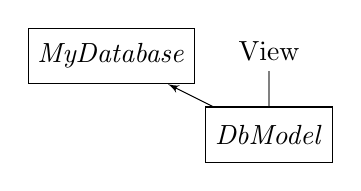
\begin{tikzpicture}[node distance=2.0cm,auto,>=latex']
            \node [int] (a) {$\mathit{MyDatabase}$};
            \node [int,below=1cm,pin={[init]above:View}] (b) [right of=a] {$\mathit{DbModel}$};
            \path[->] (b) edge node {} (a);
            \end{tikzpicture} & $\qquad \Leftrightarrow \qquad$ &
            
            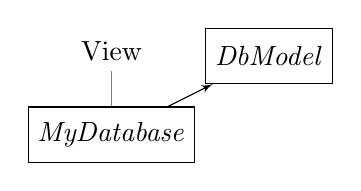
\begin{tikzpicture}[node distance=2.0cm,auto,>=latex']
            \node [int,pin={[init]above:View}] (c)  {$\mathit{MyDatabase}$};
            \node [int,above=1cm] (d) [right of=c] {$\mathit{DbModel}$};
            \path[->] (c) edge node {} (d);
            \end{tikzpicture} \\
            $\mathit{DbModel}$ object & & $\mathit{MyDatabase}$ object
        \end{tabular}
        \egroup
    \end{center}
    \caption{Cast between an $\mathit{DbModel}$ object and an $\mathit{MyDatabase}$ object} \label{fig:cast}
\end{figure}

The implementation of the illustrated cast is given below. This $\mathit{cast}$ function is part of a type class for which there are instances for every pair of sub-class and ancestor.
\begin{displaymath}
\begin{array}{lcl}
\multicolumn{3}{l}{\mathit{cast} :: \mathit{DbModelObj} \to \mathit{MyDatabaseObj}} \\
\mathit{cast}~(\mathit{DbModelEnd}~(\mathit{MyDatabaseData}~\mathit{pd})~\mathit{d}) & = & \\ \multicolumn{3}{l}{\quad \mathit{MyDatabaseStart}~\mathit{pd}~(\mathit{DbModelData}~d)} \\
\mathit{cast}~(\mathit{DbModelMiddle}~(\mathit{MyDatabaseData}~\mathit{pd})~\mathit{d}~\mathit{sub}) & = & \\ \multicolumn{3}{l}{\quad \mathit{MyDatabaseStart}~\mathit{pd}~(\mathit{DbModelStart}~d~\mathit{sub})}
\end{array}
\end{displaymath}
Casts in the other direction require a bit more work. Firstly, we need a different casting function whose result is wrapped in $\mathit{Maybe}$ to indicate that a cast from a base-class to a sub-class may not succeed. However, due to the use of existential types, we also require runtime type information about the type of the value in \emph{e.g.} the $\_\mathit{MyDatabase}\_\mathit{sub}$ field. Haskell's $\mathit{Typeable}$ type class\footnote{\url{https://hackage.haskell.org/package/base/docs/Data-Typeable.html}} may be used for this purpose.

\section{Translation}
\label{sec:auto}

Encoding object classes for our system by hand is both repetitive and error-prone. Luckily, the encoding is also well-suited for auto-generation using Template Haskell.
In this section, we propose syntactic sugar resembling the usual notation for object classes used by object-oriented languages. The corresponding encodings can automatically be generated from this syntax. Since the $\mathbf{class}$ keyword is already used for type classes in Haskell, object classes use the $\mathbf{state}$ keyword instead.
Declarations for object classes have syntax:
\begin{displaymath}
\begin{array}{l}
[\mathbf{abstract} \mid \mathbf{final}]~\mathbf{state}~\mathit{C}~\overline{\mathit{tyvar}}~[: P~\overline{\mathit{type}}]~\mathbf{where} \\
\quad \overline{\mathbf{data}~\mathit{var}~[= \mathit{expr}] :: \mathit{type}} \\
\quad \overline{[\mathbf{abstract}]~\mathit{var} :: \mathit{type}} \\
\quad \overline{\mathit{equation}}
\end{array}
\end{displaymath}
We use the usual overline and square-bracket meta-syntax for repetition
and optional elements respectively.
The $\mathbf{state}$ keyword is optionally preceded by either an $\mathbf{abstract}$ or $\mathbf{final}$ modifier, but cannot have both. If the $\mathbf{abstract}$ modifier is specified, the class cannot be instantiated directly, but it may include method typings marked as $\mathbf{abstract}$ which do not have an accompanying binding. Unless a class which inherits from an abstract class is abstract itself, it must implement all of its ancestors' methods which are marked as $\mathbf{abstract}$ and are therefore lacking an implementation. If a class is marked as $\mathbf{final}$, then no other class can inherit from it. This is accomplished by omitting the data constructors which allow successor $\Delta$-objects as shown in Figure \ref{tab:baseconstructors}.

The name of an object class $C$ follows the conventions for type constructors\footnote{In Haskell, this means that the name must start with an upper-case character.} and is followed by zero or more type variables. The optional $: \mathit{P}~\overline{\mathit{type}}$ component of the header of the declaration is used to specify the class's parent. $P$ must be the name of a non-final object class. There must be as many $\mathit{type}$s as there are type parameters in $P$'s definition. Any type variables used here must first be declared as type parameters of $C$.

The body of an object class declaration following the $\mathbf{where}$ keyword consists of three types of definitions which may appear in any order. A line starting with the $\mathbf{data}$ keyword is used to declare a field and must consist of at least a name and a type, but may optionally have an expression describing its default value. If no default value is specified, then it is assumed to be $\bot$. The fields in the object class declaration are desugared into fields for the state date type: 
\begin{displaymath}
\begin{array}{lcl}
\mathbf{data}~\mathit{CState}~\overline{\mathit{tyvar}} & = & \mathit{MkCState}~\{~\overline{\_\mathit{var} :: \mathit{type}}~\}
\end{array}
\end{displaymath}
The names of this data type and its single constructor can be chosen arbitrarily, since they are never exposed directly to the user. However, for consistency, we have used the name of the object class followed by $\mathit{State}$ for the name of the data type and $\mathit{Mk}$, followed by the name of the data type, for the constructor. This data type is parametrised over the same type parameters as $C$. The type alias for the state monad transformer parametrised over $\mathit{CState}$ follows:
\begin{displaymath}
\mathbf{type}~\mathit{C}~\overline{\mathit{tyvar}} = \mathit{StateT}~(\mathit{CState}~\overline{\mathit{tyvar}})~[\mathit{Identity} \mid PM~\overline{\mathit{type}}]
\end{displaymath}
By convention, the type alias is named after the object class. As with the state data type before, its type parameters are the same as in the header of the declaration for $C$. If the class has a parent, its underlying monad is that corresponding to $P$ applied to the type argument specified in the header of $C$. Otherwise, it is $\mathit{Identity}$. The last new type that results from a declaration for an object class $C$ is the data type representing objects of type $C$:
\begin{displaymath}
\mathbf{data}~\mathit{C}~\overline{\mathit{tyvar}} = \mathit{constructors}
\end{displaymath}
We refer to Figure \ref{tab:baseconstructors} for guidance on which constructors are depending on whether $C$ is a sub-class or not and which attributes it has. The $\mathit{Middle}$ constructor combines all possible fields which may be required by an object's internal state:
\begin{displaymath}
\begin{array}{l}
\forall s~d.\mathit{CLike}~s~d~(\mathit{C}~\overline{\mathit{tyvar}})~\overline{\mathit{tyvar}} \Rightarrow \mathit{CMiddle}~\{\\
\quad \begin{array}{lcl}
\_\mathit{C}\_\mathit{sup}  & :: & \mathit{PObject}~\overline{\mathit{type}}, \\
\_\mathit{C}\_\mathit{data} & :: & \mathit{CState}~\overline{\mathit{tyvar}}, \\
\_\mathit{C}\_\mathit{sub}  & :: & s~\overline{\mathit{tyvar}}
\end{array}\\
\}
\end{array}
\end{displaymath}
The existentially-quantified type variables $s$ and $d$ as well as the type class constraint are only required if the $\mathit{sub}$ field is present. $s$ refers to the object type of a sub-class and $d$ refers to the corresponding state type. The constraint enforces that the sub-class must implement all methods of $C$. The $\mathit{sup}$ field is only present in sub-classes, but never base classes. Its value is a $\Delta$-object belonging to $P$. Finally, the $\mathit{data}$ field is always present and stores the $\Delta$-object's state.

Method typings and fields are used to construct the type class representing $C$'s interface: 
\begin{displaymath}
\begin{array}{l}
\mathbf{class}~[\mathit{Monad}~m \mid \mathit{PLike}~o~s~m~\overline{\mathit{type}}] \Rightarrow \\
\quad \mathit{CLike}~o~s~m~\overline{\mathit{tyvar}} \mid o \to s, s \to o~\mathbf{where} \\
\qquad \begin{array}{l}
\_\mathit{C}\_\mathit{invoke} :: \mathit{CLike}~o'~d'~(\mathit{StateT}~(s~\overline{\mathit{tyvar}})~m)~\overline{\mathit{tyvar}} \Rightarrow \\
\qquad o'~\overline{\mathit{tyvar}} \to \\ \qquad (o'~\overline{\mathit{tyvar}} \to \mathit{StateT}~(s~\overline{\mathit{tyvar}})~m~(r,o'~\overline{\mathit{tyvar}})) \to\\\qquad
o~\overline{\mathit{tyvar}} \to m~(r,o~\overline{\mathit{tyvar}},o'~\overline{\mathit{tyvar}}) \\
\overline{\_\mathit{ext}\_\mathit{get}\_\mathit{field} :: o~\overline{\mathit{tyvar}} \to m~(\mathit{type}, o~\overline{\mathit{tyvar}}) } \\
\overline{\_\mathit{int}\_\mathit{get}\_\mathit{field} :: \mathit{StateT}~(s~\overline{\mathit{tyvar}})~m~\mathit{type}} \\
\overline{\_\mathit{ext}\_\mathit{set}\_\mathit{field} :: o~\overline{\mathit{tyvar}} \to \mathit{type} \to m~((),o~\overline{\mathit{tyvar}})} \\
\overline{\_\mathit{int}\_\mathit{set}\_\mathit{field} :: \mathit{type} \to \mathit{StateT}~(s~\overline{\mathit{tyvar}})~m~()} \\
\overline{\_\mathit{ext\_method} :: o~\overline{\mathit{tyvar}} \to \overline{\mathit{arg} \to}~m~(\mathit{result},o~\overline{\mathit{tyvar}})}\\
\overline{\_\mathit{int\_method} :: \overline{\mathit{arg} \to}~ \mathit{StateT}~(s~\overline{\mathit{tyvar}})~m~\mathit{result} }
\end{array}
\end{array}
\end{displaymath}

For each field, there is a getter and a setter. Just like methods, each has an internal and an external version. Note that we treat getters and setters as state transformers, just like methods. We take the view that they are \emph{properties} as they are found in \emph{e.g.} C\#. That is, while we have the expectation that a getter gets the value of a field and that a setter sets the value of the field, both can also potentially be implemented as arbitrary methods with matching types. Additionally, the $\_\mathit{C}\_\mathit{invoke}$ method is used by sub-classes to invoke their own methods in a monad stack set up by $C$.

An instance of this type class is generated as well as one for each type class belonging to an ancestor of $C$. Each external method's implementation pattern matches on the configuration of the object, adds a state monad transformer layer on top of the existing monad stack, and then either invokes its own, internal implementation of the method or propagates the call to a sub-class.

If $C$ is not a base class, a second instance of $\mathit{CLike}$ is generated with the underlying monad set to $\mathit{Identity}$. In this case, all methods use $\_P\_\mathit{invoke}$ on the $\Delta$-object belonging to $P$ to perform the process shown in Figure \ref{fig:invoke}:
\begin{displaymath}
\begin{array}{l}
\mathbf{instance}~\mathit{CLike}~\mathit{C}~\mathit{CState}~\mathit{Identity}~\overline{\mathit{tyvar}}~\mathbf{where}\\
\quad \begin{array}{lcl}
\mathit{method}~(\mathit{CEnd}~\mathit{sup}~\mathit{d}) & = & \mathbf{do} \\
\multicolumn{3}{l}{\quad \begin{array}{lcl}
    (r,sup',\mathit{CEnd}~\_~d') & \leftarrow & \\ 
    \multicolumn{3}{l}{ \quad \_P\_\mathit{invoke}~(\mathit{CEnd}~\mathit{sup}~d)~\mathit{method}~\mathit{sup} }\\
    \multicolumn{3}{l}{\mathit{return}~(r, \mathit{CEnd}~sup'~d')}
    \end{array}}
\end{array}
\end{array}
\end{displaymath}
%Methods are mostly standard Haskell. $<:$ and $>:$ statements are desugared into calls to the appropriate getters or setters for a field. Method invocations (identifiers containing dots) are rewritten so that the object becomes the first argument of the method and the resulting expression is then wrapped into $\mathit{runIdentity}$.

\section{Template Haskell}
\label{sec:th}

We have developed a Haskell library\footnote{\url{https://github.com/mbg/monadic-state-hierarchies} on GitHub and \url{http://hackage.haskell.org/package/msh} on Hackage} which implements the automatic translation from a simple object-oriented language to the encoding shown in Section \ref{sec:auto}. Object classes can be defined inside of a Haskell source file with the help of a Template Haskell $\mathit{QuasiQuoter}$\cite{mainland2007s}. The example for a simple expression language we have shown in Section \ref{sec:encoding} using Java syntax can easily be converted into our state declarations:
\begin{displaymath}
\begin{array}{l}
[\mathit{state}\mid\\\mathbf{abstract}~\mathbf{state}~\mathit{Expr}~\mathbf{where} \\
\quad \begin{array}{lcl}
\mathit{eval} & :: & \mathit{Int}\\
\end{array}\\\\
\mathbf{state}~\mathit{Add} : \mathit{Expr}~\mathbf{where} \\
\quad \begin{array}{lcl}
\mathbf{data}~\mathit{left} & :: & \mathit{Expr} \\
\mathbf{data}~\mathit{right}  & :: & \mathit{Expr}
\end{array}\\\\
\quad \begin{array}{lcl}
\mathit{eval} & :: & \mathit{Int}\\
\mathit{eval} & = & \mathbf{do} \\
\multicolumn{3}{l}{\quad  \begin{array}{lcl}
x & \leftarrow & \mathit{this}.!\mathit{left}.!\mathit{eval}\\
y & \leftarrow & \mathit{this}.!\mathit{right}.!\mathit{eval}\\
\multicolumn{3}{l}{\mathit{return}~(x + y) }
\end{array}} 
\end{array}\\
\mid]
\end{array}
\end{displaymath}
The quotation is parsed and then translated into an abstract representation of Haskell's syntax, according to the rules shown in Section \ref{sec:auto}. Method typings must be given, similar to type classes. We parse them as standard Haskell, but their co-domains will be wrapped into \emph{e.g.} $\mathit{AddM}$ in the example above. Method equations are also parsed as normal Haskell, but no transformations are applied. The code for this and other examples may be found in our code repository.

\subsection{Selectors}

In order to allow programmers to work with the object classes, our library contains a number of combinators. Most of these combinators operate on \emph{selectors} which are defined using a GADT and are indexed over whether they represent a mutable member, \emph{i.e.} a field, or an immutable member, \emph{i.e.} a method. The $\mathit{MemberType}$ type is promoted to the kind level and the $\mathit{Mutable}$ and $\mathit{Immutable}$ constructors are used as types:
\begin{displaymath}
\begin{array}{l}
\mathbf{data}~\mathit{MemberType} = \mathit{Mutable} \mid \mathit{Immutable} \\\\
\mathbf{data}~\mathit{Selector}~(\mathit{ty} :: \mathit{MemberType})~o~s~m~a~\mathbf{where} \\
\quad \begin{array}{lcl}
 \mathit{MkMethod} & :: & \mathit{StateT}~s~m~a \to \\
                   &    & (o \to m~(a, o)) \to\\
                   &    & \mathit{Selector}~\mathit{Immutable}~o~s~m~a \\
\mathit{MkField}   & :: & (o \to m (a,o)) \to \\
                   &    & \mathit{StateT}~s~m~a \to \\
                   &    & (o \to a \to m~((),o)) \to \\
                   &    & (a \to \mathit{StateT}~s~m~()) \to \\
                   &    & \mathit{Selector}~\mathit{Mutable}~o~s~m~a
\end{array}
\end{array}
\end{displaymath}
Intuitively, a selector is a value which contains both, internal and external, versions of a member so that the same name can be used for both. For fields, it contains both versions for the getter and the setter. 
The type classes which are generated for object classes contain selectors for all of their members, using the original names from the state declaration. For example, including inherited members and in addition to the type class methods shown in Section \ref{sec:auto}, the $\mathit{Add}$ object class contains:
\begin{displaymath}
\begin{array}{l}
\mathit{left} :: \mathit{AddLike}~o~s~m \Rightarrow \\
\qquad \mathit{Selector}~\mathit{Mutable}~o~s~m~\mathit{Expr} \\
\mathit{right} :: \mathit{AddLike}~o~s~m \Rightarrow \\
\qquad \mathit{Selector}~\mathit{Mutable}~o~s~m~\mathit{Expr} \\
\mathit{eval} :: \mathit{EvalLike}~o~s~m \Rightarrow \\
\qquad \mathit{Selector}~\mathit{Immutable}~o~s~m~\mathit{Int} \\
\end{array}
\end{displaymath}
Selectors allow us to use member names directly in either an internal or external call context without any compile-time transformations which resolve them to the appropriate functions. For example, in the type class instance for $\mathit{Add}$, $\mathit{left}$ has the following value:
\begin{displaymath}
\mathit{left} = \mathit{MkField}~\mathit{\_ext\_get\_next}~\mathit{\_int\_get\_next}~\mathit{\_ext\_set\_next}~\mathit{\_int\_set\_next}
\end{displaymath}

\subsection{Selector composition}

In object-oriented languages, member access can be chained together using the $.$ ``operator''. For example, $\mathit{obj}.\mathit{foo}.\mathit{bar}$ gets the value of a field $\mathit{foo}$ belonging to an object $\mathit{obj}$ and then invokes the $\mathit{bar}$ method on the value of $\mathit{foo}$. We have a similar mechanism in our library. However, since $.$ is already used for function composition, we use $.!$ instead. This operator is part of a type class $\mathit{Object}$, which is added as a super-class constraint to every type class generated for the interface of a base class:
\begin{displaymath}
\begin{array}{l}
\mathbf{infixr}~8~.!\\
\mathbf{class}~\mathit{Monad}~m \Rightarrow \mathit{Object}~\mathit{obj}~\mathit{st}~m~\mathit{where} \\
\qquad \begin{array}{lcl}
\mathit{this} & :: & \mathit{This}~\mathit{obj}~\mathit{st}~\mathit{m}~\mathit{obj} \\
\mathit{this} & = & \mathit{MkThis} \\\\

(.!) & :: & \forall r~\mathit{ty}.\\ 
     &    & \mathit{obj} \to \\
     &    & \mathit{Selector}~\mathit{ty}~(\mathit{QueryObject}~\mathit{obj})~\mathit{st}~(\mathit{QueryMonad}~\mathit{obj}~\mathit{m})~r \to  \\
     &    & \mathit{QueryResult}~\mathit{obj}~\mathit{ty}~\mathit{st}~m~r
\end{array}
\end{array}
\end{displaymath}
Note that the $\mathit{This}$ type is defined as $\mathbf{data}~\mathit{This}~o~s~m~a = \mathit{MkThis}$ and simply serves to capture the type arguments of instances of the $\mathit{Object}$ type class. The type of $.!$ is highly flexible. The left argument of the operator can be any type that is made an instance of the $\mathit{Object}$ class. Primarily, those are objects as the name would imply, but selectors and $\mathit{This}$ are also instances of $\mathit{Object}$. The right argument is always a selector. We use the $\mathit{QueryObject}$ and $\mathit{QueryMonad}$ type families to determine what object the selector will be accessing and what monad stack it will run on, depending on the left argument of $.!$.

The $.!$ operator is right-associative so that we can build up larger selectors and ultimately decide whether the call should be internal or external, depending on whether we apply it to an object or $\mathit{this}$.

The type of selector we obtain from composing two selectors is determined by a closed type function:
\begin{displaymath}
\begin{array}{l}
\mathbf{type}~\mathbf{family}~\mathit{MemberComposeResult} \\
\quad (\mathit{lhs} :: \mathit{MemberType})~(\mathit{rhs} :: \mathit{MemberType} :: \mathit{MemberType})~\mathbf{where} \\\\
\qquad \begin{array}{lcl}
\mathit{MemberComposeResult}~\mathit{Immutable}~\mathit{Immutable} & = & \mathit{Immutable} \\
\mathit{MemberComposeResult}~\mathit{Immutable}~\mathit{Mutable} & = & \mathit{Immutable} \\
\mathit{MemberComposeResult}~\mathit{Mutable}~\mathit{Immutable} & = & \mathit{Immutable} \\
\mathit{MemberComposeResult}~\mathit{Mutable}~\mathit{Mutable} & = & \mathit{Mutable} 
\end{array}
\end{array}
\end{displaymath}
Intuitively, the result of composing two selectors can only be a mutable selector if both of the original selectors are also mutable. 

In most object-oriented languages, $\mathit{null}$ is automatically a value of all reference types. Members of a field or variable can be accessed without checking whether the value is $\mathit{null}$ or not, frequently leading to runtime errors which are difficult to track down. Functional languages, such as ML or Haskell, do not have $\mathit{null}$ values -- they have a better solution: the option type. In Haskell, this type is called $\mathit{Maybe}$ and is defined as:
\begin{displaymath}
\begin{array}{lcl}
\mathbf{data}~\mathit{Maybe}~a & = & \mathit{Nothing} \mid \mathit{Just}~a
\end{array}
\end{displaymath}
In other words, a value of type $\mathit{Maybe}~a$ is either $\mathit{Nothing}$ -- the rough equivalent of $\mathit{null}$ -- or $\mathit{Just}~x$ for some $x :: a$. Case analysis must be performed on every such value to determine whether it contains a value of type $a$ or not. Functions expecting an argument of type $a$ cannot be applied to a value of type $\mathit{Maybe}~a$. Object-oriented languages have recently begun to adapt this type as a type-safe alternative in favour of $\mathit{null}$. However, checking whether a value is $\mathit{Nothing}$ or not can still be tedious if, for example, we wish to only run some function if a certain value is not $\mathit{null}$. C\#, for example, has recently introduced the $.?$ operator which can be used in place of $.$. The member on the right of $.?$ will only be accessed if the value on the left is not the equivalent of $\mathit{Nothing}$.

As functional programmers, we know that C\#'s $.?$ operator is really just a specialised version of $\mathit{fmap}$, because the option type is a functor. In our library, we have a $.\$$ operator in addition to $.!$, which fulfils the same role as C\#'s $.?$ operator, except that it is not specialised to the option time. Instead, it works for any type that is an instance of the $\mathit{Functor}$ type class. We believe that this is further evidence that, by combining ideas from both paradigms, we can 

\subsection{Combinators}

Field selectors can be assigned new values in the definition of a method using the $<:$ operator. It is defined as follows: 
\begin{displaymath}
\begin{array}{l}
(<:)  ::  \mathit{Monad}~m \Rightarrow \mathit{Selector}~\mathit{Mutable}~o~s~m~\mathit{val} \to \mathit{val} \to \mathit{StateT}~s~m~()\\
(\mathit{MkField}~\_~\_~\_~s') <: val  =  s' val
\end{array}
\end{displaymath}
Note that method selectors cannot be supplied as an argument to $<:$ since we explicitly require the selector to be tagged as $\mathit{Mutable}$. Haskell's type system then ensures that this is adhered to.

Every external call returns a pair consisting of a result as well as an updated object. A language like Java would just mutate the object on which the external call was made, but since our system is pure and values are immutable, this cannot be done. Surrounding external calls with $\mathit{fst}$ and $\mathit{snd}$ may seem a bit cryptic, so instead we provide aliases named $\mathit{result}$ and $\mathit{object}$ for the projections, respectively. 

We will often want to perform case analysis on the value of a member within a method. Instead of first binding the value to a variable and then using $\mathbf{case}$ on it, we provide a shortcut. The $\mathit{switch}$ combinator has type $\mathit{Monad}~m \Rightarrow \mathit{Selector}~\mathit{ty}~o~s~m~\mathit{val} \to (\mathit{val} \to \mathit{StateT}~s~m~b) \to \mathit{StateT}~s~m~b$.

As an example of these combinators, consider an implementation of linked lists in the object-oriented style:

\begin{displaymath}
\begin{array}{l}
\mathbf{state}~\mathit{ListItem}~a~\mathbf{where} \\
\qquad \begin{array}{lcl}
\mathbf{data}~\mathit{value} & :: & a \\
\mathbf{data}~\mathit{next}  & :: & \mathit{Maybe}~(\mathit{ListItem}~a)
\end{array}\\\\
\qquad \begin{array}{lcl}
\mathit{appendEnd} & :: & \mathit{ListItem}~a \to () \\
\mathit{appendEnd}~\mathit{item} & = & \mathbf{do} \\
 \multicolumn{3}{l}{\qquad \begin{array}{lcl}
abc&&
\end{array}}
\end{array}
\end{array}
\end{displaymath}

\subsection{Normal type classes}

Objects generated by our library can be made instances of ``normal'' Haskell type classes, removing the need for object-oriented-style interfaces. For example, we could write the following to make $\mathit{Val}$ objects an instance of the $\mathit{Show}$ type class:
\begin{displaymath}
\begin{array}{l}
\mathbf{instance}~\mathit{Show}~\mathit{Val}~\mathbf{where}\\
\qquad \begin{array}{lcl}
\mathit{show}~\mathit{obj} & = & \mathit{show}~(\mathit{result}~(\mathit{obj}.!\mathit{value})) 
\end{array}
\end{array}
\end{displaymath}
We believe that this, together with the flexibility of selectors, shows that our system is not an entirely different world from existing Haskell code, but can be used in combination with it.


\section{Related work}
\label{sec:related}

Extending Haskell with an object system is not a new idea. Previous work evaluated various approaches to constructing object systems within Haskell and emphasised encoding information about object classes in the type system~\cite{kiselyov2005haskell}, which our encoding does not. Their library supports many of the principal features of object-oriented languages, but uses IO references to accomplish this while we wish to remain pure. There has also been work to allow Haskell to interact with object-oriented languages more easily, such as a language extension allowing object-oriented-style overloading in Haskell~\cite{shields2001object}. Type classes are also used to establish a subtyping relation. However, their work does not allow object-oriented style code to be written in Haskell itself.

The popular \texttt{lens} library by Edward Kmett\footnote{\url{https://hackage.haskell.org/package/lens}} and similar other libraries provide types and combinators for the traversal and manipulation of data structures. A $\mathit{Lens}$ combines a getter and setter for a field, similarly to our selectors. Lenses can be composed to traverse nested data structures.
Combining lenses with our encoding of objects (future work)
would enable the vast number of combinators in the \texttt{lens} library to be used on top of our system.

While most programming languages with object-oriented features are impure, theoretical backing for our system comes from formalisations of pure object calculi based on the $\lambda$-calculus~\citet{pierce1994simple}. Methods in this system are state transformers like in ours, taking objects as arguments and returning updated objects. We believe that the explicitness of a purely-functional object system allows for more flexibility than the implicitness of an impure system.

%In more theoretical work,~\cite{Pierce93simpletype-theoretic} present A typed $\lambda$-calculus with support for encapsulation, message passing, subtyping, and inheritance is presented by. Methods in this calculus are state transformers, but they do not form stacks of state monad transformers. Instead, methods simply use the object as state as in traditional object-oriented programming.

The expression problem is concerned with the choice between different ways in which programs may be extended with new functionality without having to change any of the existing code. A classical example of this is wishing to extend a programming language with new features without having to change any existing code. Our example in Section \ref{sec:encoding} demonstrates how this can partially be approached in our system. We have also drawn an analogy between the expression problem and the ``monad transformer problem''. 

Other approaches to modular data types exist for Haskell as well. Open data types and functions is a proposed extension for Haskell which enables data types and functions to be marked as ``open''. A data type marked with this keyword allows new constructors and function equations to be added after the initial declaration. This is accomplished by generating normal data types and functions from all open declarations within a program. While this approach has the advantage that it does not introduce any fundamentally new concepts to the language, it does require whole-program compilation and changes the order in which pattern matching occurs~\cite{loh2006open}.

Modular data types can be constructed in Haskell without any new extensions to the type system using the \emph{data types \`a la carte technique}~\cite{swierstra2008data}. Unlike open data types, it does not require whole-program compilation, but instead it requires a stronger grasp of the underlying techniques. To the authors' knowledge, there is no simple notation for the \`a la carte technique. This technique has been used to construct \emph{e.g.} modular compilers in which independent language fragments can introduce effects to the overall language~\cite{day2012towards}. It is not clear how easily effects can be interleaved in our system, since we assume a fixed ordering of effects.

%One alternative to the monad transformer library called \emph{Monatron}~\cite{jaskelioff2011monatron} which features an improved lifting mechanism at the cost of increased implementation complexity improves upon the \texttt{mtl} library, but shifts the difficulty from library users to library authors. \emph{Monad zippers} and \emph{monad views}~\cite{schrijvers2011monads} which are used to hide and address parts of monad stacks respectively provide another interesting approach to dealing with the complexity of monad transformers.

%One of the most promising solutions so far has been presented in~\cite{kiselyov2013extensible} where a single monad, parametrised over a set of effect handlers~\cite{plotkin2009handlers} is used to implement an effect system in Haskell. The order of effects is not fixed on the type-level, but is determined on the value level. This system is also more efficient than monad transformers since it only needs to find a matching handler when a given effect is required. Monad transformers, on the other hand, always execute all of their effects between computations, even if most of them are not required.

\section{Conclusions and future work}
\label{sec:conclusions}

We have shown how several concepts in object-oriented programming related to concepts in functional programming. Most notably, we have established a link between monad transformers and inheritance. In order to take advantage of this connection, we have encoded an object system based on state monad transformers in pure Haskell. Our encoding also has a notation of coercive subtyping which allows for the construction of modular data types in Haskell. Additionally, we have described a process for translating to our encoding from a simple object-oriented language. This process is implemented in a Haskell library, enabling programmers to use object classes in their Haskell programs without having to resort to a different language or impurity. Almost all of the types in our system can be inferred, with the only exceptions of method types and the results of $\mathit{new}$.

The type classes which support the inheritance mechanism hide calls to the $\mathit{lift}$ function of monad transformers from the programmer, while also allowing more fine-grained control through the opportunity for method overriding. Each layer of our monad stack is mapped to a corresponding object class. We believe that this is a powerful representation of monad transformers which we plan to explore further in future work to allow for non-state classes.

A major limitation of our encoding compared to popular object-oriented languages is the lack of aliasing. While we do not believe that aliasing is an essential feature of an object system, it is often considered a key feature of object-oriented programming. Unfortunately, it requires references to an object to be shareable so that an update through one can be observed through the others -- a side effect. In impure languages, this is accomplished by storing all objects in a global heap, but this makes reasoning about such programs difficult. A good compromise may be the introduction of localised heaps which are shared between all functions which possess an alias to the same object. This may be accomplished with the help of the $\mathit{ST}$ monad \cite{launchbury1995state} which provides local, mutable state in Haskell. Such a system would not only improve our encoding, but matches similar efforts in object-oriented languages to better encapsulate objects -- see, for example, the essay by Hogg\cite{hogg1992geneva} on controlling object aliasing or ownership types\cite{clarke1998ownership}.

Outside of the context of Haskell, it may also be interesting to design a language with an object system for effect in mind. This could lead to a simpler representation of objects through corresponding language support, potentially leading to greater computational efficiency. However, we have not yet investigated how our encoding performs. 





\subsubsection*{Acknowledgments.} We would like to thank the anonymous referees and Dominic Orchard for their valuable feedback on an earlier versions of this paper. This work was supported by EPSRC.

%TODO: these need to be embedded and properly formatted for the springer format
\bibliographystyle{abbrv}
\bibliography{pwmsh}

\end{document}
